% !TEX root = ../thesis.tex

\chapter{Introduction}\label{sec:introduction}

Super resolution microscopy has become, with recent developments, a fundamental source of data in the field of biology. On top of this, imaging techniques like \textsc{palm} have been combined with single-particle tracking\mcite{palm2008}, allowing to reconstruct thousands of simultaneous particle trajectories at increasingly high spatiotemporal resolution. With the availability of this large quantity of information, new data analysis techniques are needed to extract relevant biophysical features that can give new insights on the biological processes. Existing knowledge from physics and mathematics can provide a solid base to build a toolset of statistical and analytical methods to accomplish this goal. Langevin's equation and stochastic processes, for example, have been extensively---and successfully---used to model the dynamics of biological systems\mcite{schuss2010}. Likewise, regression and unsupervised learning algorithms represent a powerful tool to classify the large amount of data produced by single-particle tracking. Valuable insights can be obtained by carefully joining data driven methods and theoretical modelling. Either approaches are valid but may not be sufficient, per se, to reveal the inner significance of certain processes; their combination can instead provide hints about the deeper mechanisms of life. Redundancy, for example, seems to be a fundamental principle in many biological processes, as the joint application of narrow escape model and numerical simulations has suggested\mcite{reynaud2015, schuss2017, basnayake2018}. Yet to be understood problems in biology can benefit hugely from this twofold approach. Gathering of high resolution datasets paves the way to new and promising discoveries. On the other hand, data is useless without a solid framework to analyse and explain it. Overwhelming availability of data can even be counterproductive, as it makes the extraction of meaningful patterns more complicated. Dealing with these challenges is going to be, in the very near future, one of the major efforts in all fields of scientific research.

In this thesis I will present some results regarding data analysis, modelling and numerical simulations based on single-particle tracking data. The \textit{fil rouge} connecting the whole work is the search for explanation of the dynamics of amyloid beta (Aβ) aggregates in neurons, which are known to be involved in Alzheimer's disease\mcite{AD}. In this introduction I will briefly review the current knowledge about Alzheimer's and the main techniques in super resolution microscopy. In chapter \ref{sec:data_analysis} I will present the analysis of \textsc{spt} data. While the dataset used specifically regards Aβ aggregates, the final aim is to build a general methodological framework to allow the extraction of biophysical features from \textsc{spt} recordings in different contexts. Following the results of the data analysis, in chapter \ref{sec:modelling} I will reformulate the initial hypothesis and focus on a model of motion\mcite{holcman2018single} involving the endoplasmic reticulum (\textsc{er}), describing the results of numerical simulations that I developed to better understand the biological implications of the model.
% that has been developed by Holcman's team\mcite{holcman2018single} based on the analysis of the Aβ data,

\section{Alzheimer's disease}\label{sec:alzheimer}

Alzheimer’s disease is the most common form of dementia in elder adults. As population ages, the death rate due to the disease is steadly increasing. Statistics published by the Centres for Disease Control and Prevention show that Alzheimer’s-related deaths in \tsc{USA} increased 55\% between 1999 and 2014, making it the sixth leading cause of death. The disease causes a progressive loss of brain functions (neuron deaths) to a point where it impaires basic cognitive skills. Most common symptoms are memory loss and language impairement.

As of today, causes of the Alzheimer’s are not fully understood by the scientific community. Despite several clinical trials, no treatment has been proved to be---even partially---effective in treating the disease. Most scientists agree that probably there is no single cause for Alzheimer’s, but a combination of several genetic and environmental factors.

\fxwarning{Add references}

\subsection{The amyloid hypothesis}

\begin{figure}
  \sidecaption{\tolerance=20 Illustration representing Aβ placques inside the brain (shown as brown spherical aggregates between neurons). \emph{Image courtesy of the National Institute on Aging/NIH.}\label{fig:plaques}}
  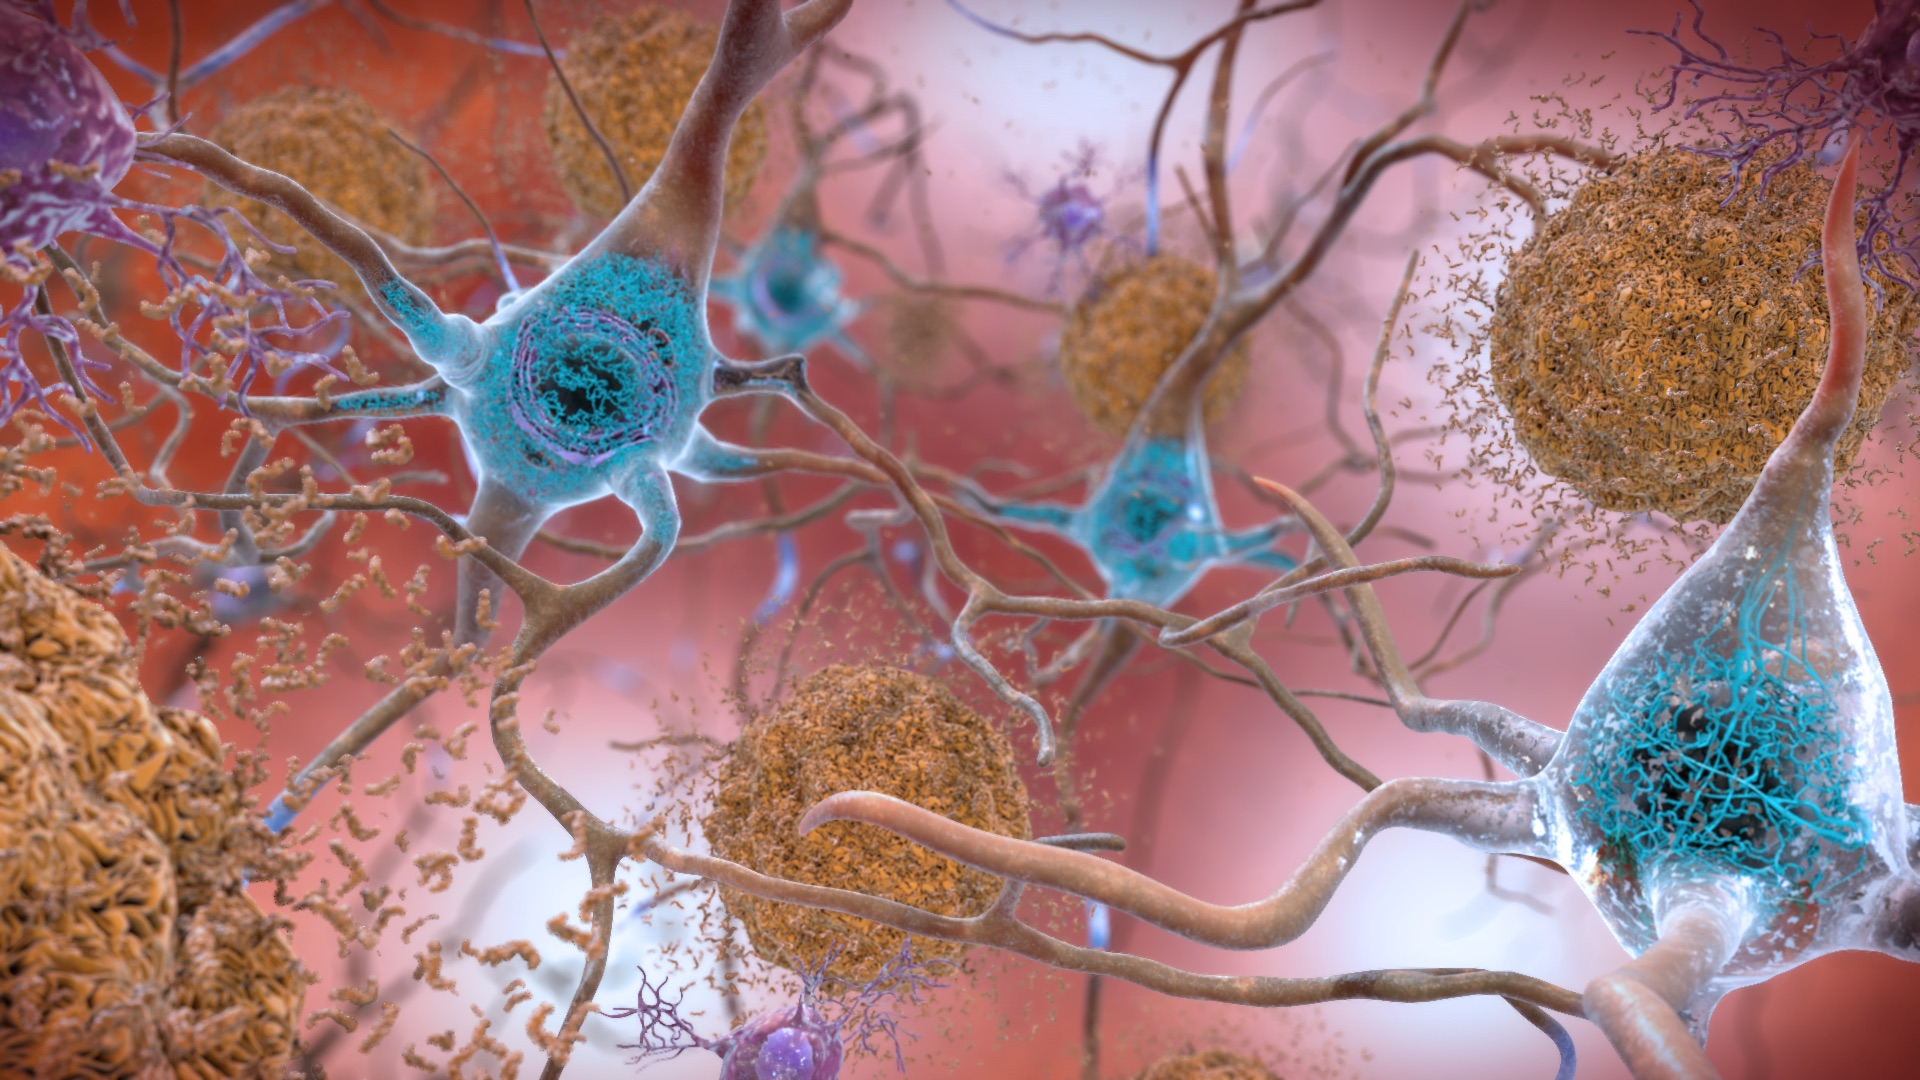
\includegraphics[width=\textwidth]{nia_plaques.jpg}
\end{figure}

A long standing attempt to explain Alzheimer’s disease is the \emph{amyloid hypothesis}. One of the most distinctive characteristics of people affected by the disease is the formation of amyloid-β (Aβ) aggregates in the brain extracellular space (\cref{fig:plaques}).
These clumps, known as \emph{plaques}, are thought to start a cascade process leading to brain inflammation, cells deaths and synapses dysfunction. Despite solid evidence proving the association between Alzheimer's disease and Aβ plaques, the amyloid hypothesis didn't lead to any beneficial result in terms of medical therapy. Various treatments targeting Aβ aggregates have been trialled but, even if successful in dissolving plaques, no effect on patients' cognitive functions has been observed. The general explanation of these disappointing results is that treatments are administered too late in the disease progression, when plaques have already activated an uncontrollable cascade of damaging processes. Supporting this idea, it has been shown that formation of Aβ plaques can begin decades before the manifestation of symptoms. Despite being often criticised for its failures, the amyloid theory remains one of the main directions in Alzheimer's disease research.


\section{Super resolution microscopy and single-particle tracking}

We will look at Alzheimer's disease from a very small scale, studying the motion of amyloyd-β inside neural cells. Observing these kind of biological samples at molecular scale requires a very high resolution. In particular, one has to capture details beyond the light diffraction limit. The ensemble of techniques that allow to overcome this limit is known as \emph{super resolution microscopy}. In the context of wide-field flourescence imaging, two main strategies exist to achieve super resolution. The first and more traditional one is using patterned light illumination techniques such as \emph{structured imaging microscopy} (\tsc{SIM})\mcite{sim1995}. \tsc{sim} relies on Moiré patterns created by illuminating the sample through different gratings. The patterns can then be analysed in reciprocal space to reconstruct the high resolution image. The second strategy is more recent and consists in localisation based methods such as \emph{photo-activated localization microscopy} (\tsc{PALM})\mcite{palm2006,palm2008} and \emph{stochastic optical reconstruction microscopy} (\tsc{STORM})\mcite{storm2006}. Both \tsc{palm} and \tsc{storm} work by selectively activating subsets of fluorophores to avoid diffraction effects between closely spaced samples. This is obtained through \emph{photobleaching} (the spontaneous fading of the flourophore) in \tsc{PAML} and by \emph{photoswitching} (the controlled switching between on/off states) in \tsc{STORM}.

All these techniques have undergone a remarkable development in recent years, making it possible to capture super resolution images at small time intervals (in the order of tens of milliseconds). These recordings allow to observe the motion of single molecules in cells at nanometer scale. In practice, one can reconstruct the molecules trajectories by linking their position observed in consecutive frames. Several tools and techniques have been designed to perform this operation\mcite{saxton2008}, that goes under the name of \emph{single-particle tracking} (\tsc{SPT}). The advantage of \tsc{SPT} data with respect to other methods is that it measures individual molecule dynamics (and not just ensemble averages). Although the method is limited by the imaging time resolution, it allows to perform a much fine-grained analysis than other ensemble-based techniques.

\begin{figure}
  \sidecaption{A frame taken from a fast \tsc{SIM} recording. Bright spots are amyloid beta aggregates moving inside a cell. The trajectory of one of them (circled in red) obtained by \tsc{SPT} is shown in green.\label{fig:tracking}}
  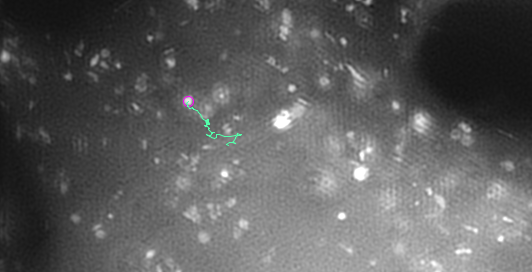
\includegraphics[width=\textwidth,height=6.5cm]{tracking.png}
\end{figure}
